% language syntax and the compiler, the notions of locality and parallelism and how they are orthogonal
% concepts in Chapel

\section{Chapel base language}
\chapter{Chapel base language}
\subsection{} % creates page markers at the top

\begin{frame}{Why another language?}
\end{frame}

\begin{frame}{Exercise: using functions and control flow}
  Write a Chapel code to find the root of the equation $x^5 + 8x^3 - 2x^2 + 5x - 1.2 = 0$ using the bisection
  method in the interval [-1,1]
  \begin{columns}[]
    \column{0.45\textwidth}
    \begin{itemize}\setlength{\itemsep}{3mm}
      \item Calculate the function at the ends and the midpoint of the interval
      \item Depending on the signs of the three computed values, let the midpoint be either the new left
      or the new right end
      \item Repeat until your error is below $\Delta x=10^{-8}$
    \end{itemize}
    \column{0.55\textwidth}
    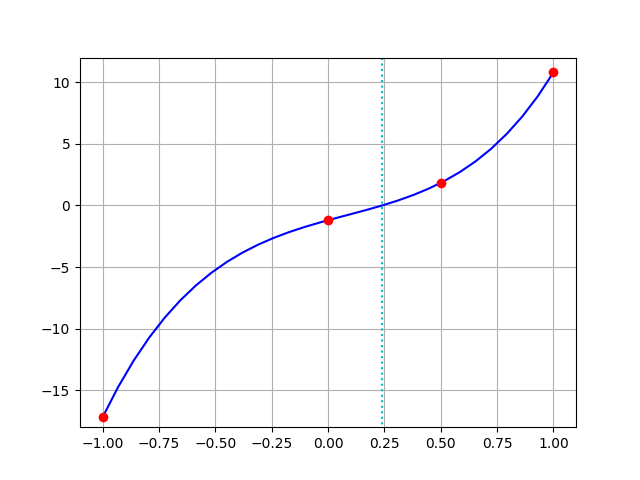
\includegraphics[width=0.95\columnwidth]{figs/bisection.png}
  \end{columns}
\end{frame}
